\chapter{Theoretical formalism and numerical realization}
\label{formalism}
All results in this work have been obtained in momentum space by resorting to partial-wave decomposition (PWD) what is convenient for calculations in the framework of the Faddeev equations. We use the non-relativistic formalism, neglect the Coulomb force and 3N interaction.
%The potentials used in this work have been constructed to be used in the non-relativistic formalism.
%Since the OPE-Gaussian force was derived in coordinate space, the additional transformation of its matrix elements from coordinate space to momentum space was done. This was achieved by the standard transformation formula which requires numerical integrations involving spherical Bessel functions.
\section{2N bound state}
\label{calculation}
%\subsection{Calculating 2N bound states}
%\label{calcbound}
The Hamiltonian of two-nucleon systems can be written in general form
\begin{equation}
H^{(2)} = H^{(2)}_{0} + V_{\mathrm{2N}}\;,
\end{equation}
where $H^{(2)}_{0}$ is the kinetic energy of two nucleons and $V^{(2)}_{\mathrm{2N}}$ is the NN potential. The kinetic energy of the two-particle system is
\begin{equation}
H^{(2)}_{0} = \frac{\vec{\!{\,p}}^{2}_{1}}{2m_{1}} + \frac{\vec{\!{\,p}}^{2}_{2}}{2m_{2}} = \frac{\vec{\!{\,p}}^{2}}{2\mu} + \frac{\vec{\!{\,\mathcal{P}}}^{2}}{2M}\;,
\label{eqHam1}
%\frac{\boldsymbol{\hat{{p_{1}}}}^{2}}{}
\end{equation}
where $\mu = \frac{m_{1}m_{2}}{m_{1}+m_{2}}$ is the reduced nucleon mass and $M = m_{1} + m_{2}$. Using the average nucleon mass $m_{1}$ = $m_{2}$ = $m = \frac{2m_{p}m_{n}}{m_{p} + m_{n}}$ we have the relative momentum $\vec{p}  = \frac{m_{1}\vec{p}_{2} - m_{2}\vec{p}_{1}}{m_{1} + m_{2}} = \frac{1}{2}\left(\vec{p}_{2} - \vec{p}_{1}\right)$ and $\!\vec{\,\mathcal{P}} = \!\!\vec{\,p}_{1} + \!\vec{\,p}_{2}$ the total momentum for two nucleons. 

The deuteron bound wave function $\ket{\Psi_{d}}$ is a solution of the time-independent Schr{\"o}dinger equation
\begin{equation}
\left(H^{(2)}_{0} + V_{\mathrm{2N}}\right)\left|\Psi_{\mathrm{d}}\right> = E_{d}\left|\Psi_{\mathrm{d}}\right>\;,
\end{equation}
where $E_{d} < 0$. Using Eq.~(\ref{eqHam1}) and assuming that $V_{\mathrm{2N}}$ depends only on the relative degrees of freedom leads to two separated equations
\begin{equation}
\frac{\!\vec{\,p}^{2}}{m}\braket{\vec{p}}{\Psi_{d}}
+ \int\limits_{0}^{\infty}\mathrm{d}\!\vec{\,p}^{\prime} \left<\!\vec{\,p}^{\prime}|V_{\mathrm{2N}}|\!\vec{\,p}\right>
\braket{\!\vec{\,p}^{\prime}}{\Psi_{d}} = \left(E_{d} - E_{\mathrm{c.m.}}\right)\braket{\!\vec{\,p}}{\Psi_{d}}\;,
\label{eqHam2}
\end{equation}
and
\begin{equation}
\frac{\!\vec{\mathcal{\,P}}^{2}}{2m}\left<\!\vec{\mathcal{\,P}}|\Psi_{d}\right> = E_{\mathrm{c.m.}}\left<\!\vec{\mathcal{\,P}}|\Psi_{d}\right>\;.
\label{eqHami3}
\end{equation}
Since the total momentum of the system is conserved, the relative energy of the center of mass between two nucleons, $E_{\mathrm{c.m.}}$, equals zero (deuteron is at rest) and the equation~(\ref{eqHami3}), which describes the free motion of a particle with mass $M$, is omitted.

We use the momentum partial-wave representation
\begin{equation}
\begin{split}
&\ket{p\alpha_{2}} \equiv \ket{p(ls)jm_{j}}\ket{tm_{t}}\;,\\
\end{split}
\label{eqalpha2}
\end{equation}
where $p\equiv |\!\vec{\, p}|$ is the magnitude of the relative momentum, and $\alpha_{2}$ is a set of discrete quantum numbers describing 2N system $\ket{\alpha_{2}} \equiv \ket{(ls)jm_{j}} \ket{tm_{t}}$, where $l$, $s$, $j$, and $t$ denote the orbital angular momentum, total spin, total angular momentum, and total isospin of 2N system, respectively. Further $m_{j}$ ($m_{t}$) are the projections of $j$ ($t$) onto quantization axis. The coupling of above-mentioned quantum numbers is given by
%the total angular momentum onto the spin $\left|sm_{s}\right|$ correspond to 2N spin states with the total spin 0 and 1;. The coupling of 
%%All these quantities are projected on the axis $\hat{z}$, where the spin (isospin) of each nucleon is coupled with corresponded the total spin (isospin) of 2N systems, respectively. More explicitly it can be represented by
\begin{equation}
\begin{split}
&\ket{p(ls)jm_{j}} = \sum\limits_{m_{l}}c(lsj;m_{l},m_{j}-m_{l},m_{j})\ket{plm_{l}}\ket{sm_{j}-m_{l}}\;,\\
&\ket{sm_{s}} = \sum\limits_{m_{1} = -1/2}^{1/2}C\left(\frac{1}{2},\frac{1}{2}, s;m_{1},m_{s}-m_{1},m_{s}\right)\ket{\frac{1}{2}m_{1}}\ket{\frac{1}{2}m_{s}-m_{1}}\;,\\
&\ket{tm_{t}} = \sum\limits_{\nu = -1/2}^{1/2}C\left(\frac{1}{2},\frac{1}{2}, t;\nu,m_{s}-\nu,m_{t}\right)\ket{\frac{1}{2}\nu}\ket{\frac{1}{2}m_{t}-\nu}\;,
\end{split}
\end{equation}
where $m_{l}$ is the projection of the orbital angular momentum. Further, spin states $\ket{sm_{s}}$ correspond to 2N spin states with the total spin 0 or 1; $C(j_{1}, j_{2}, j; m_{1}, m_{2}, m)$ denote the Clebsch-Gordan coefficients. Similarly, $\ket{tm_{t}}$ is the ispospin state. We assume for individual particles the isospin projection $\nu = \frac{1}{2}$ for proton and $\nu = - \frac{1}{2}$ for neutron. 

The 2N states are antisymmetric as for a system of two identical fermions, which leads to one more constraint on quantum numbers $l$, $s$ and $t$
\begin{equation}
(-1)^{l+s+t} = -1\;.
\end{equation}

The partial-wave states (\ref{eqalpha2}) fulfills
\begin{equation}
\left<\!\vec{\, p}^{\prime}|plm_{l}\right> = \frac{\delta (p - p^{\prime})}{pp^{\prime}}Y_{lm_{l}}(\theta,\phi)\;,
\end{equation}
where $Y_{lm_{l}}(\theta,\phi)$ denotes the spherical harmonic function with angles $\theta, \phi$ pointing direction of momentum $\vec{p}$~\cite{edmonds}. The completeness relation for $\left|p \alpha_{2}\right>$ states is expressed as
\begin{equation}
\sum\limits_{\alpha_{2}}\int\limits_{0}^{\infty}\mathrm{d}p p^{2}\ket{p\alpha_{2}}\bra{p\alpha_{2}} = \mathbbm{1}\;.
\end{equation}
%which leads to the fact that we need infinitely many $\ket{\alpha_{2}}$ states. 
%In all my practical calculations, one can restrict to a finite number of basis vectors by setting the total angular momentum of the 2N system as $j_{\mathrm{max}} \geq 0 $. 

%Depending on a given kinematics $j_{\mathrm{max}}$, we have $N_{\alpha_{2}} = 2 + 4j_{\mathrm{max}}$ 2N states, in this work I used $j_{\mathrm{max}} = 5$, in principle, this is sufficient to describe the 2N scattering observables and the deuteron properties.
\begin{table}[]
\centering
\begin{tabular}{|l|l|l|l|l|l|l|}
\hline
        & N$^{2}$LO & N$^{3}$LO & N$^{4}$LO & N$^{4}$LO$^{+}$ & OPEG & Exp.~\cite{van1982deuteron} \\ \hline
$E_{d}$ [MeV] 
&\multicolumn{1}{l|}{\begin{tabular}[c]{@{}l@{}}-2.1999\\$\pm$0.0041\end{tabular}}
&\multicolumn{1}{l|}{\begin{tabular}[c]{@{}l@{}}-2.2233\\$\pm$0.0024\end{tabular}}
&\multicolumn{1}{l|}{\begin{tabular}[c]{@{}l@{}}-2.2233\\$\pm$0.00099\end{tabular}}           
&\multicolumn{1}{l|}{\begin{tabular}[c]{@{}l@{}}-2.2233\\$\pm$0.0012\end{tabular}}                 
&\multicolumn{1}{l|}{\begin{tabular}[c]{@{}l@{}}-2.2225\\$\pm$0.00001\end{tabular}}
&\multicolumn{1}{l|}{\begin{tabular}[c]{@{}l@{}}-2.2246\\$\pm$0.0092\end{tabular}}      \\ \hline
$P(^{3}S_{1})$ [\%] 
&\multicolumn{1}{l|}{\begin{tabular}[c]{@{}l@{}}95.3665\\$\pm$0.0041\end{tabular}}
&\multicolumn{1}{l|}{\begin{tabular}[c]{@{}l@{}}95.3034\\$\pm$0.0024\end{tabular}}
&\multicolumn{1}{l|}{\begin{tabular}[c]{@{}l@{}}95.4633\\$\pm$0.00099\end{tabular}}           
&\multicolumn{1}{l|}{\begin{tabular}[c]{@{}l@{}}95.4114\\$\pm$0.0012\end{tabular}}                 
&\multicolumn{1}{l|}{\begin{tabular}[c]{@{}l@{}}94.6987\\$\pm$0.0412\end{tabular}}
&\multicolumn{1}{l|}{\begin{tabular}[c]{@{}l@{}}---\end{tabular}}      \\ \hline
\end{tabular}
\caption{The deuteron binding energy $E_{d}$ with the statistical uncertainty (see text in Chapter~\ref{statistical}) obtained with various NN interactions.}
\label{tabgs}
\end{table}
The only two deuteron components $^{3}S_{1}$- and $^{3}D_{1}$ (we use the standard notation $^{2s+1}l_{j}$), corresponds to $l$ = 0 and $l$ = 2, respectively, with $s = j = 1$ and $t$ = $m_{t}$ = 0. This leads to two coupled equations
\begin{equation}
\frac{p^{2}}{m}\psi_{l}(p)
+ \sum\limits_{l^{\prime}, l = 0}^{2}\int\limits_{0}^{\infty} dp^{\prime}p^{\prime 2}\left<p l|V_{\mathrm{2N}}|p^{\prime}l^{\prime}\right> \psi_{l^{\prime}}(p^{\prime}) = E_{d}\psi_{l}(p)\;,
\label{eqHam2}
\end{equation}
for the partial-wave components of the deuteron wave function $\psi_{l}(p) = \braket{pl}{\psi_{d}} = \bra{p(l1)1m_{d}}\braket{00}{\psi_{d}}$.
%$\ket{pl} \equiv \ket{p(l1)1m_{d}}\ket{00}$, $\psi_{l}(p) \equiv \braket{pl}{\Psi_{d}}$. 
The integral (\ref{eqHam2}) can be discretized using the Gaussian quadrature with Gaussian points and weights ($p_{j}, w_{j}$) with $j = 1, 2, \ldots, N_{p}$ distributed in the finite interval $(0, \bar{p})$, where the upper limit of the integration, $\bar{p}$ has to be adjusted to the used NN potential $V_{\mathrm{2N}}$. Than, Eq. (\ref{eqHam2}) expresses as
\begin{equation}
\frac{p^{2}_{i}}{m}\psi_{l}(p_{i})
+ \sum\limits_{l^{\prime} = 0}^{2}\sum\limits_{j = 1}^{N_{p}} w_{j}p^{\prime 2}_{j}\left<p_{i} l|V_{\mathrm{2N}}|p_{j}l^{\prime}\right> \psi_{l^{\prime}}(p_{j}) = E_{d}\psi_{l}(p_{i})\;.
\label{eqHam3}
\end{equation}
%For example, employing a numerical integration by the Gaussian quadrature rule with the upper limit of the integration, $\bar{p}$, depending on the NN potential
%The integral can then be discretized using quadrature and the resulting algebraic system be
%For a numerical treatment of Eq. (C.3) we assume that the
%integral over $p_{0}$ is carried out with some choice of Gaussian points and weights ($p_{j}, w_{j}$)
%with $j = 1, 2, \ldots, N_{p]$ distributed in the finite interval $(0, p̄)$, where the upper limit of the
%integration, $\bar{p}$, might depend on the nucleon-nucleon potential used.
We solve the resulting an eigenvalue problem, using the FORTRAN code together with the LAPACK library and compute the deuteron wave function and the deuteron binding energy, $E_{d}$. The deuteron binding energy computed with the chiral SMS potentials at various chiral orders with cutoff $\Lambda$ = 450 MeV and with the OPE-Gaussian force is given in Table~\ref{tabgs}.
% for chiral potential disagree with the values in Ref.~\cite{Reinert2018} is explained due to differences choice of Gaussian points and weights in numerical treatment used for Eq. (\ref{eqHam3}).
\begin{figure}
\center{\includegraphics[width=1.\textwidth,clip=true]{PhD-text/4_Formalism/deuwf.eps}} 
%\includegraphics[width=5.3cm]{PhD-text/4_Formalism/deuwf.eps}
%\includegraphics[width=5.3cm]{PhD-text/4_Formalism/deuwf.eps}
\caption{The deuteron wave functions in momentum $\Psi_{l}(p)$ space. The $^{3}S_{1}$ and the $^{3}D_{1}$ components are shown in the left and right columns, respectively. The black solid, blue dashed, red dashed-dotted, orange dashed-dot-dotted and green dotted curves are for the chiral N$^{2}$LO, N$^{3}$LO, N$^{4}$LO, N$^{4}$LO$^{+}$ and the OPEG potentials, respectively.}
\label{fig:deuwf}
\end{figure}
In the final step the deuteron wave functions $\psi_{0}(p)$ and $\psi_{2}(p)$ require normalization via
\begin{equation}
\int\limits_{0}^{\infty}dp p^{2}\left(\psi^{2}_{0}(p) + \psi^{2}_{2}(p)\right) = 1\;.
\end{equation}
In Figure~\ref{fig:deuwf} I show the $^{3}S_{1}$- and $^{3}D_{1}$-states obtained by using the chiral N$^{2}$LO, N$^{3}$LO, N$^{4}$LO, N$^{4}$LO$^{+}$ SMS forces and the OPE-Gaussian potential. It can be seen that all predictions almost coincide with each other. The magnitude of $^{3}S_1$-state is nearly 70 times bigger than in $^{3}D_1$-state. The corresponding $^{3}S_1$-component probability is given in the bottom row of Table~\ref{tabgs}.

%The $^{3}D_1$ component of the OPE-Gaussian deuteron wave function is more differs from the remaining predictions, but not critically. 

%In addition, for further calculations, for example, three-nucleon reactions, one can need the deuteron state $\ket{\Psi_{d}m_{d}}$ which in the above-mention basis (\ref{eqalpha2}) is given by
%\begin{equation}
%\begin{split}
%\ket{\Psi_{d}m_{d}} &= \sum_{\alpha_{2}}\int\limits_{0}^{\bar{p}}\mathrm{d}pp^{2}\ket{p\alpha_{2}}\braket{p\alpha_{2}}{\Psi_{d}m_{d}} = \\
%&= \int\limits_{0}^{\bar{p}}\mathrm{d}pp^{2}\left(\ket{p(01)1m_{d}\ket{00}}\psi^{2}_{0}(p) + \ket{p(21)1m_{d}\ket{00}}\psi^{2}_{2}(p)\right)\;.
%\end{split}
%\end{equation}
%A description of how to compute the deuteron wave function $\psi_{l} (p)$ numerically is given in Appendix A.
%\begin{figure}[ht]
%\begin{minipage}[h]{0.495\linewidth}
%\center{\includegraphics[width=1.\textwidth,clip=true]{PhD-text/4_Formalism/deuwf_3S1.eps}}    \\
%\end{minipage}
%\hfill
%\begin{minipage}[h]{0.495\linewidth}
%\center{\includegraphics[width=1.\textwidth,clip=true]{PhD-text/4_Formalism/deuwf_3D1.eps}} 
%\end{minipage}
%\caption{The five-fold cross section $\frac{d^{5}\sigma}{d\Omega_{1}d\Omega_{2}dS}$ for the $d(n,n_{1}n_{2})p$ 
%breakup reaction at the incoming nucleon laboratory kinetic energy $E$=~65~MeV for the following 
%directions momenta of outgoing neutrons: a) $\theta_{1} = 30.5^{\circ}, \theta_{2} = 59.5^{\circ}, \phi_{12} = 180^{\circ}$ (QFS configuration) and b) $\theta_{1} = \theta_{2} = 54.0^{\circ}, \phi_{12} = 120^{\circ}$ (SST configuration). 
%The orange, green and violet bands represent statistical uncertainties obtained with the OPE-Gaussian force, the chiral N$^{4}$LO and N$^{4}$LO+ ($\Lambda~=~450$~MeV), respectively. The experimental data are from Ref.~\cite{Allet} for a) and from Ref.~\cite{Zejma} for b).}
%\label{fig} 
%\end{figure}

%Introducing the following complete set of 2N momentum states that will be
%used in further calculations
%We work in the formalism of partial wave decomposition and introduce the momentum space basis of partial wave states $\mid p, \alpha_{2}\rangle$ and $\mid p, q, \alpha\rangle$ for the two-nucleon and three-nucleon states, respectively~\cite{glockle1983quantum, Glockle1996}. Here  $p \equiv|p_{1}|$ is the magnitude of the relative momentum of two nucleons (nucleons 2 and 3 in the three-nucleon case), and $q \equiv|q_{1}|$ is the magnitude of the momentum of the spectator nucleon with respect to the center of mass of nucleons 2 and 3. The Jacobi momenta $p_{i}$ and $q_{i}$ ($i = 1, 2, 3$) can be expressed by the momenta of individual nucleons $k_{i}$. Further, $\alpha_{2}$ is a set of discrete quantum numbers describing two-nucleon system and is given as $|\alpha_{2}\rangle\equiv|(ls)jm_{j}; tm_{t}\rangle$ where $l, s, j$, and $m_{j}$ are the orbital angular momentum, total spin of two nucleons, the total angular momentum, and its projection on the quantization axis, respectively. The isospin part is described by the total two-body isospin $t$ and its projection $m_{t}$. For three-nucleon state $\alpha$ represents the set of quantum numbers in the so-called $jI$-coupling, and is defined as $|\alpha\rangle\equiv|(ls)j, (\lambda,1/2)I (jI)JM_{J}; (t, 1/2)TM_{T}\rangle$. Here $l,s, j$ and $t$ describe two-nucleon subsystem (2-3). Next, $\lambda$ is the orbital angular momentum of nucleon 1, which together with its spin 1/2, couples to the total angular momentum $I$. The angular momenta $j$ and $I$ couple finally to the total angular momentum of the 3N system $J$, and $M_{J}$ denote its projection on the quantization axis. The quantum numbers $T$ and $M_{T}$ describe, the total isospin of the 3N system and its third component, respectively. 
%%Index 1 indicates that the quantum numbers in the two-body subsystem are for particles 2 and 3.
%
%To compute the deuteron binding energy $E_{d}$  and the deuteron wave function $\psi_{d}$ the Schr{\"o}dinger equation $\mathrm{H \psi_{d} = E_{d} \psi_{d}}$ is used.
%In the case of two-nucleon system, the Schrödinger equation H ψd = Ed ψd is used to compute the deuteron binding energy Ed  and the deuteron wave function ψd . The standard techniques to solve the eigenproblem is also used.
%\subsubsection{Deuteron}
%In the case of two-nucleon system there is only one bound state formed by a neutron and a proton the non-relativistic Schr{\"o}dinger equation 
%\subsection{Calculating 2N scattering observables}
%Epelbaum2015 Epelbaum2015a, Reinert

%The first two types of regularization were tested and compared in Refs.~\cite{Skibinski2018, }

%outlined briefly in Section

%\section{Error propagation from NN potentials}
\section{2N scattering}
\label{LSE}
In this chapter I introduce the essential components of 2N scattering calculations. I start with a discussion of the Lippman-Schwinger equation for the scattering state in momentum space. Solving it in terms of the transition matrix ($t$-matrix) by realizing its PWD one gets the half-the-energy-shell amplitude (half-shell amplitude). Next, I obtain $K$-matrix, which in turn, is related to the scattering matrix $S$-matrix. $S$-matrix can be further expressed in terms of a linear combination of Wolfenstein parameters that allowed us to compute observables, e.g. the cross-section and various polarization observables at various energies.
%, in the following will be denoted as $E_{\mathrm{lab}}$
\subsection{The Lippman-Schwinger equation in PWD}
The scattering state $\ket{\Psi_{\vec{p}}}$ of two particles in momentum space, fulfils the time-independent Schr{\"o}dinger equation
\begin{equation}
\left(H_{0} + V_{\mathrm{2N}}\right)\ket{\Psi_{\vec{p}}} = E\ket{\Psi_{\vec{p}}}\;,
\label{eqLSE}
\end{equation}
with $E > 0$. Its solution fulfils the Lippman-Schwinger equation
\begin{equation}
\ket{\Psi_{\vec{p}}} = \ket{\Psi_{0}} + \frac{1}{E - H_{0} \pm i\varepsilon}V_{\mathrm{2N}}\ket{\Psi_{\vec{p}}}\;,
\label{eqLSE01}
\end{equation}
with $\varepsilon \rightarrow 0^{+}$. If we write down (\ref{eqLSE01}) in coordinate representation, we will get two parts of the solution --- a spherical outgoing wave ($+i\varepsilon$) or a plane incoming wave ($-i\varepsilon$)~\footnote{``-$i\varepsilon$"-states appear, for example, in the photodisintegration process ($\gamma$ + $^{2}$H $\rightarrow n + p$).}, see Refs.~\cite{glockle1983quantum, ChElsterLecs} for more details. The state $\ket{\Psi_{0}}$ is momentum eigenstate 
\begin{equation}
\ket{\Psi_{0}} \equiv \ket{\!\vec{\,p}}~\mathrm{with}~\frac{\!\vec{\,p}^{2}}{2\mu} = E\;,
\end{equation}
where $\vec{p}$ is the relative momentum of the two nucleons and $E$ depends on the incoming nucleon energy in the laboratory reference frame~\footnote{Given $E_{\mathrm{lab}}$ and assuming that $m_{p}$ = $m_{n}$ = $m$, each nucleon in the c.m.s. has a relative momentum which refers to an unknown $E \equiv E_{\mathrm{cm}} = \frac{\!\vec{\, p}^{2}}{m}$. In turn, $E = E_{\mathrm{lab}} - \frac{\!\vec{\, p}^{2}}{2(2m)} = \frac{1}{2}E_{\mathrm{lab}}$.}. The solution of Eq. (\ref{eqLSE01}) can be denoted as $\ket{\Psi_{\!\vec{\,p}}}= \ket{\!\vec{\,p}}^{+}$.
%It should also be noted that we are dealing with a time-independent problem, but the time-dependence is known to us in the form $\ket{\!\vec{\,p}}^{+}e^{-iEt}$. 

Eq. (\ref{eqLSE01}) can be rewritten as
\begin{equation}
\ket{\!\vec{\,p}}^{+} = \ket{\!\vec{\,p}} + \tilde{G}_{0}(E + i\varepsilon)V_{\mathrm{2N}}\ket{\!\vec{\,p}}^{+}\;,
\label{eqLSE1}
\end{equation} 
where $V \equiv V_{\mathrm{2N}}$ and the free propagator
\begin{equation}
\tilde{G}_{0}(E) \equiv \frac{1}{E - H_{0}}\;.
%+ i\varepsilon
\end{equation} 
Using the definition of the transition operator ($t$-matrix)
\begin{equation}
V\ket{\!\vec{\,p}}^{+} = t^{+}\ket{\!\vec{\,p}}\;,
\end{equation}
and substituting it into Eq.~(\ref{eqLSE1}) we find
\begin{equation}
\begin{split}
&V\ket{\!\vec{\,p}}^{+} = V\ket{\!\vec{\,p}} + V\tilde{G}_{0}(E + i\varepsilon)V\ket{\!\vec{\,p}}^{+}\;,
\end{split}
\end{equation}
and thus
\begin{equation}
\begin{split}
&t^{+}\ket{\!\vec{\,p}} = V\ket{\!\vec{\,p}} + V\tilde{G}_{0}(E + i\varepsilon)t^{+}\ket{\!\vec{\,p}}\;.
\end{split}
\end{equation}
The latter equation is the form of the Lippman-Schwinger equation for the operator $t^{+}$
\begin{equation}
t^{+} = V + V\tilde{G}_{0}(E + i\varepsilon)t^{+}\;.
\label{eqt}
\end{equation}
%To construct the on-shell amplitude $T = \left<\!\vec{\, p}^{\prime}|V|\vec{p}\right>^{+}$  
%It is more convenient to consider $H = H_{0} + V$ in terms of the free propagator $\tilde{G}_{0}(E)$ and the full propagator $\tilde{G}(E) = \frac{1}{E - H}$ to emphasize the structure of the $t$-matrix element from a certain choice of the initial condition and the final state. Thus,
%\begin{equation}
%\begin{split}
%\tilde{G}^{-1}_{0}(E) &= \tilde{G}^{-1}(E) + V\;\\
%\tilde{G}^{-1}(E) &= \tilde{G}^{-1}_{0}(E) + \tilde{G}^{-1}(E)V\tilde{G}^{-1}_{0}(E)~\mathrm{or}\\
%\tilde{G}^{-1}(E) &= \tilde{G}^{-1}_{0}(E) + \tilde{G}^{-1}_{0}(E)V\tilde{G}^{-1}(E)\;.
%\label{EqGE}
%\end{split}
%\end{equation}
%Using $V\tilde{G}(E) = t(E) \tilde{G}_{0}(E)$ one can get
%\begin{equation}
%\begin{split}
%t(E) = V + V\tilde{G}_{0}(E)t(E)\;.
%\end{split}
%\label{eqte}
%\end{equation}
Note that in general case Eq. (\ref{eqt}) can be iterated for scattering on $V$ 
\begin{equation}
\begin{split} 
t &= V + V\tilde{G}_{0}V + V\tilde{G}_{0}V\tilde{G}_{0}V + V\tilde{G}_{0}V\tilde{G}_{0}V\tilde{G}_{0}V + \ldots\;,
\end{split}
\end{equation}
this is so-called von Neumann series. Finally one can express $\ket{\vec{p}}^{+}$ through the $t$-matrix
\begin{equation}
\ket{\!\vec{\,p}}^{+} = \ket{\!\vec{\,p}} + \tilde{G}_{0}(E + i\varepsilon)t(E + i\varepsilon)\ket{\!\vec{\,p}}
\end{equation}
%%central transition matrix elements of scattering theory
%
Considering the $t$-matrix for general states $\ket{\!\vec{\,p}^{\prime}}$, $\ket{\!\vec{\,p}}$, which obeys the Lippman-Schwinger equation (\ref{eqLSE01}), we get the off-the-energy-shell amplitude~\cite{glockle1983quantum}
\begin{equation}
\begin{split}
\left<\!\vec{\,p}^{\prime}|t(E + i\varepsilon)|\!\vec{\,p}\right> &= 
\left<\!\vec{\,p}^{\prime}|V(E + i\varepsilon)|\!\vec{\,p}\right> \\
&+\lim\limits_{\varepsilon \rightarrow 0^{+}}\int\limits_{0}^{\infty}\mathrm{d}\!\vec{\,p}^{\prime\prime}\left<\!\vec{\,p}^{\prime\prime}|V(E + i\varepsilon)|\!\vec{\,p}\right>\frac{\left<\!\vec{\,p}^{\prime}|t|\!\vec{\,p}\right>}{E_{p^{\prime}} + i\varepsilon - E_{p^{\prime\prime}}}\;,
\end{split}
\label{Eqtmain}
\end{equation}
where $E_{p^{\prime}} = \frac{|\!\vec{\,p}^{\prime}|^{2}}{m}$ and $E_{p^{\prime\prime}} = \frac{|\!\vec{\,p}^{\prime\prime}|^{2}}{m}$. 
%Using the Cauchy principal value (PV) of a finite integral of a function, the Green's function can be separated into its real and imaginary parts
%\begin{equation}
%\lim\limits_{\varepsilon\rightarrow 0^{+}}\frac{1}{E_{p^{\prime}} + i\varepsilon - E_{p^{\prime\prime}}} = PV \frac{1}{E_{p^{\prime}} - E_{p^{\prime\prime}}} - i\pi\delta (E_{p^{\prime}} - E_{p^{\prime\prime}})\;.
%\end{equation}
In a similar manner as has been done for the deuteron, PWD projection of Eq. (\ref{Eqtmain}) onto the same complete set of basis state (\ref{eqalpha2}) and using the upper limit for the $p^{\prime\prime}$ integration, $\bar{p}$, results in
\begin{equation}
\begin{split}
&\left<p^{\prime}\alpha^{\prime}_{2}|t|p\alpha_{2}\right> = \left<p^{\prime}\alpha^{\prime}_{2}|V|p\alpha_{2}\right> + \\& \sum\limits_{l^{\prime\prime} = j-1, j+1}\lim\limits_{\varepsilon \rightarrow 0^{+}}\int\limits_{0}^{\bar{p}}\mathrm{d}p^{\prime\prime}
\frac{p^{\prime\prime 2}
\left<p^{\prime\prime}\alpha^{\prime}_{2}|V|\!\vec{\,p}\right>\left<p^{\prime}\alpha^{\prime}_{2}|t|p\alpha_{2}\right>}{E_{p^{\prime}}- E_{p^{\prime\prime}} + i\varepsilon }\;,
\end{split}
\label{Eqtmain2}
\end{equation}
%The integral can then be discretized using quadrature and the resulting algebraic system be
%For a numerical treatment of Eq. (C.3) we assume that the
%integral over $p_{0}$ is carried out with some choice of Gaussian points and weights ($p_{j}, w_{j}$)
%with $j = 1, 2, \ldots, N_{p]$ distributed in the finite interval $(0, p̄)$, where the upper limit of the
%integration, $\bar{p}$, might depend on the nucleon-nucleon potential used.
%Imposing restriction related to energy conservation into the $t$-matrix
%\begin{equation}
%\frac{\!\vec{\,p}^{\prime}}{m} = \frac{\!\vec{\,p}}{m}
%\end{equation}
%we get the one-the-energy-shell amplitude (the on-shell amplitude), which allows us to calculate the cross section.
The $t$-matrix at $E = \frac{p^{2}}{m}$ is related to the $K$-matrix~\cite{glockle1983quantum} via
\begin{equation}
\begin{split}
t = (1 + 2i\pi \mu p K)^{-1}K\;.
\end{split}
\label{Eqkmain}
\end{equation}
and to the $S$-matrix via
\begin{equation}
\begin{split}
S = (1 + 2i\pi \mu p K)^{-1}(1 - 2i\pi \mu p K)^{-1}\;.
\end{split}
\label{EqSmain}
\end{equation}
which is used to get phase-shifts. 
%It is worth mentioning that the Coulomb interaction can be rigorously treated within the Vincent-Phatak method~\cite{Phatak} thus both neutron-proton and proton-proton scattering investigated. 
\subsection{2N scattering observables}
\label{2N}
Studying the scattering of particles with spin 1/2 allows one to carry out much more diverse measurements than only cross sections. Experiments can be made for different polarization of the beam, target and/or outgoing particles, polarized individually or simultaneously. As a result, there are $ 16 \times 16 = 256$ of various experiments, but due to the parity conservation and the time- reversal symmetry, the number of independent experiments is reduced up to 11 $np$- and 9 $pp$-measurements~\cite{glockle1983quantum}. 
%%%%% Prove it
%This leads to the fact that the 2N scattering amplitude satisfying the equation Eq. (\ref{Eqtmain2}) and the on-shell condition contains all the dynamical information about scattering. 
%%%%
The general scattering amplitude can be written as $M$-matrix and its representation is 
\begin{equation}
\begin{split}
M &= a + c\left(\!\vec{\,\sigma}_{1} + \!\vec{\,\sigma}_{2}\right)\hat{N} + m\left(\!\vec{\,\sigma}_{1}\hat{N}\right)\left(\!\vec{\,\sigma}_{2}\hat{N}\right) + (g + h)\left(\!\vec{\,\sigma}_{1}\hat{P}\right)\left(\!\vec{\,\sigma}_{2}\hat{P}\right)\\
&+(g - h)\left(\!\vec{\,\sigma}_{1}\hat{K}\right)\left(\!\vec{\,\sigma}_{2}\hat{K}\right)\;,
\end{split}
\end{equation}
where $a$, $m$, $c$, $g$ and $h$ are the Wolfenstein parameters and 
\begin{equation}
\hat{K} \equiv \frac{\!\vec{\, p}^{\prime} - \!\vec{\, p}}{|\!\vec{\, p}^{\prime} - \!\vec{\, p}|}\;,~\hat{P} \equiv \frac{\!\vec{\, p}^{\prime} + \!\vec{\, p}}{|\!\vec{\, p}^{\prime} + \!\vec{\, p}|}\;,~\hat{N} \equiv \frac{\!\vec{\, p}^{\prime} \times \!\vec{\, p}}{|\!\vec{\, p} \times \!\vec{\, p}^{\prime} |}\;.
\end{equation}
Since the $S$ -matrix contains full dynamic information, then decomposing it on partial-waves basis $S^{js}_{l^{\prime}l}$-matrix elements and taking it on-the-energy-shell allows to calculate the partial-wave elements of $M$, see Ref.~\cite{glockle1983quantum},
\begin{equation}
\begin{split}
M^{st}_{m^{\prime}_{s}m_{s}} &= \frac{1}{ip}\sum\limits_{jl^{\prime}l}C\left(l^{\prime}, s,j;m_{s} - m^{\prime}_{s},m^{\prime}_{s},m_{s}\right)Y_{l^{\prime}(m^{\prime}_{s} - m_{s})}(\theta,\phi)\\
&\times i^{l-l^{\prime}}\left(S^{js}_{l^{\prime}l} - \delta_{l^{\prime}l}\right)C\left(l, s,j;0,m_{s},m_{s}\right)\sqrt{\pi(2l + 1)}\left[1 - (-1)^{l+s+t}\right]\;.
\end{split}
\end{equation}
The partial-wave $S^{js}_{l^{\prime}l}$-matrix element is nothing else but $S^{js}_{l^{\prime}l} \equiv \left<l^{\prime}sj|S|lsj\right>$.

In the uncoupled case ($l = l^{\prime}$) the $S$-matrix can be parametrized by one phase shift
\begin{equation}
S^{js}_{ll} = e^{2i\delta_{l}}\;.
\end{equation}
For the coupled channels (for which the nuclear force allows for changes of angular momentum) the $S$-matrix is $2\times 2$ unitary and symmetric. According to the Stapp parametrisaton~\cite{Stapp} it can be written as
\begin{equation}
S = 
\left(\begin{matrix} 
\cos (2\varepsilon) \mathrm{exp}(2i\delta_{1}) & i\sin (2\varepsilon) \mathrm{exp}(i(\delta_{1} + \delta_{2})) \\
i\sin (2\varepsilon) \mathrm{exp}(i(\delta_{1} + \delta_{2})) & \cos (2\varepsilon) \mathrm{exp}(2i\delta_{2})
\end{matrix}\right)\;,
\end{equation}
where $\delta_{1}$, $\delta_{2}$ are phase shifts and $\varepsilon$ is a mixing parameter.

Using the  $M$-matrix~\cite{glockle1983quantum}, the resulting spin averaged differential cross section is given by
\begin{equation}
\frac{d\sigma}{d\Omega} = \frac{1}{4}\mathrm{Tr}\lbrace MM^{\dagger}\rbrace\;.
\label{Eq2Ncross}
\end{equation}

The polarization of one of the two particles is defined as
\begin{equation}
\begin{split}
&P = \frac{\mathrm{Tr}\lbrace MM^{\dagger}\vec{\sigma}\rbrace}{\mathrm{Tr}\lbrace MM^{\dagger}\rbrace} = \frac{8\mathrm{Re}\lbrace c^{*}(a+m)\rbrace}{\mathrm{Tr}\lbrace MM^{\dagger}\rbrace}\hat{N}\;,
\end{split}
\label{Eq2Npola1}
\end{equation}
where $\vec{\sigma}$ can be either $\!\vec{\,\sigma}_{1}$ or $\!\vec{\,\sigma}_{2}$. 
%The polarization $P$ is used to study the spin-dependence of NN force.

The remaining 2N scattering spin observables expresses as
\begin{equation}
\begin{split}
&D = \frac{\mathrm{Tr}\lbrace M(\vec{\sigma}\cdot\hat{N})M^{\dagger}(\vec{\sigma}\cdot\hat{N})\rbrace}{\mathrm{Tr}\lbrace MM^{\dagger}\rbrace}\;,\\
&R = \frac{\mathrm{Tr}\lbrace M(\vec{\sigma}\hat{N}\times \hat{p})M^{\dagger}(\vec{\sigma}\cdot\hat{K})\rbrace}{\mathrm{Tr}\lbrace MM^{\dagger}\rbrace}\;,\\
&R^{\prime} = \frac{\mathrm{Tr}\lbrace M(\vec{\sigma}\hat{N}\times \hat{p})M^{\dagger}(\vec{\sigma}\cdot\hat{P})\rbrace}{\mathrm{Tr}\lbrace MM^{\dagger}\rbrace}\;,\\
&A = \frac{\mathrm{Tr}\lbrace M(\vec{\sigma}\cdot\hat{p})M^{\dagger}(\vec{\sigma}\cdot\hat{K})\rbrace}{\mathrm{Tr}\lbrace MM^{\dagger}\rbrace}\;,\\
&A^{\prime} = \frac{\mathrm{Tr}\lbrace M(\vec{\sigma}\cdot\hat{p})M^{\dagger}(\vec{\sigma}\cdot\hat{P})\rbrace}{\mathrm{Tr}\lbrace MM^{\dagger}\rbrace}\;,
\end{split}
\label{Eq2Nall}
\end{equation}
where $\hat{p} = (\sin\theta\cos\phi, \sin\theta\sin\phi, \cos\theta)$. The observable $D$ determines the change of polarization with respect to normal direction, the depolarisation observables $R$, $R^{\prime}$, $A$, and $A^{\prime}$ determine the four possible linear combinations referring to beam and target spin polarization in scattering plane.

In the case of two polarised particles 
%one can be considered their coincidence in the final state by using parity invariance 
we find the spin-correlation coefficients, e.g.
\begin{equation}
C_{NN} = \frac{\mathrm{Tr}\lbrace MM^{\dagger}\!\vec{\,\sigma}_{1}\cdot\hat{N}\!\vec{\,\sigma}_{2}\cdot\hat{N}\rbrace}{\mathrm{Tr}\lbrace MM^{\dagger}\rbrace}\;.
\label{Eqspincorr}
\end{equation}
More detailed information about the 2N scattering observables and the partial-wave decomposition can be found in Ref.~\cite{glockle1983quantum}.
%\cite{kamada2011determination}

\section{The Faddeev equation}
\label{FaddeevEq}
%\label{LSE}
Theoretical investigations of Nd scattering can be performed within the Faddeev equations. This is one of the standard techniques to investigate 3N reactions and has been described in detail many times, see, e.g. Refs.~\cite{Witaa2001, Glockle1996, glockle1983quantum}. In following I will just briefly describe the key points of the formalism and its practical implementation.

In case of 3N system it is convenient to use the relative ($\vec{p}$ and $\vec{q}$) momenta and the total 3N momentum, $\vec{\mathcal{P}}$ represented by individual nucleon momenta $\vec{k}_{i}$, $i \in \lbrace 1,2,3\rbrace$
\begin{equation}
\begin{split}
&\vec{p} = \frac{1}{2}\left(\!\vec{k}_{2} - \!\vec{k}_{3}\right)\;,\\
&\vec{q} = \frac{2}{3}\left(\!\vec{k}_{1} - \frac{1}{2}\left(\!\vec{k}_{2} + \!\vec{k}_{3}\right)\right)\;,\\
&\vec{\mathcal{P}} = \!\vec{k}_{1} + \!\vec{k}_{2} + \!\vec{k}_{3}\;.
\end{split}
\label{eq:jacobi}
\end{equation}
The Jacobi momentum $\vec{p}$ is a relative momentum of nucleons 2 and 3 and the Jacobi momentum $\vec{q}$ is the momentum of nucleon 1 with respect to the center of mass of the 2-3 subsystem. The definition~\ref{eq:jacobi} can be extended to a more general case where the Jacobi momenta $\!\vec{\,p}_{i}$, $\!\vec{\,q}_{i}$ are used, see Figure~\ref{fig:jacobi}. We are working in 3N center of mass system what allows us to deal with 2 instead of 3 independent momenta, $\vec{\mathcal{P}} = \vec{0}$. 
\begin{figure}
\center{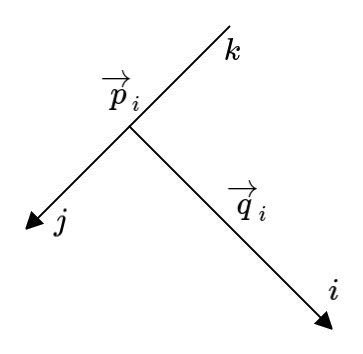
\includegraphics[width=0.3\textwidth,clip=true]{PhD-text/4_Formalism/jacobi_momenta_1.png}} 
\caption{Jacobi momenta $\vec{p}_{i}$ and $\vec{q}_{i}$ depending on suitable permutations.}
\label{fig:jacobi}
\end{figure}

The full 3N Hamiltonian reads 
\begin{equation}
H = H_{0} + V_{23} + V_{13} + V_{12} + V_{123}\;,
\end{equation}
where $H_{0} = \frac{\!\vec{\,p}^{2}}{m} + \frac{3}{4}\frac{\!\vec{\,q}^{2}}{m}$ is the free 3N Hamiltonian in the c.m. frame in terms of the Jacobi momenta, $V_{ij}$ denotes the NN potential acting between nucleons $i$ and $j$, and $V_{123}$ is the 3N potential, which can be always splitted to potential $V^{(i)}$ symmetric under the exchange of nucleons $j$ and $k$:
\begin{equation}
V_{123} = V^{(1)}_{4} + V^{(2)}_{4} + V^{(3)}_{4}\;,
\end{equation}
where $V^{(1)}_{4}$ is symmetric under the exchange of nucleons 2 and 3. In the case of three identical particles the totally antisymmetric state $\ket{\Psi}$ of three nucleons is given by
\begin{equation}
\begin{split}
\ket{\Psi} &= \ket{\psi_{1}} + \ket{\psi_{2}} + \ket{\psi_{3}} = (1+P)\ket{\psi_{1}}\;,
\end{split}
\end{equation}
where the permutation operator $P \equiv P_{12} P_{23} + P_{13} P_{23}$ is built from transmutations $P_{ij}$, which exchange particles $i$ and $j$ and $\ket{\psi_{1}}$ the Faddeev component of $\ket{\Psi}$. For example, the three-nucleon bound state $\ket{\Psi_{b}}$ fulfills the eigenvalue equation~\cite{nogga1997triton}
\begin{equation}
\ket{\psi_{1}} = G_{0} t P \ket{\psi_{1}}\;,
\end{equation}
where the two-nucleon $t$-operator obtaining by Eq.~(\ref{eqt}) acts now in the 3N space and $G_{0}$ is the free 3N propagator. For the 3N bound states, the energy argument of $G_{0}$ plays the role of the binding energy. 

The transition amplitude $U$ for the elastic Nd scattering is calculated prior to computing 3N scattering observables. Its matrix elements between the initial Nd $\ket{\phi}$ and final Nd $\ket{\phi^{\prime}}$ scattering state are given by~\cite{Glockle1996}
\begin{equation}
\begin{split}
\left<\phi^{\prime}|U|\phi\right> = \left<\phi^{\prime}|PG^{-1}_{0}|\phi\right> + \left<\phi^{\prime}|PT|\phi\right>\;.
\end{split}
\label{FaddeevElastic}
\end{equation}
For the deuteron breakup reaction the transition amplitude $U_{0}$ fulfils
\begin{equation}
\begin{split}
\left<\phi^{\prime}_{0}|U_{0}|\phi_{0}\right> = \left<\phi^{\prime}_{0}|(1 + P)T|\phi_{0}\right>\;,
\end{split}
\label{FaddeevBreakup}
\end{equation}
where $\ket{\phi^{\prime}_{0}}$ carries the information about the final free three-nucleon breakup channel.

The Faddeev equation for the auxiliary state $T\ket{\phi}$ for which nucleons interact via a NN interaction $V$ entering a $t$-matrix and a 3NF $V_{4}$ expressed as
\begin{equation}
\begin{split}
T\ket{\phi} &= t P \ket{\phi} + tP G_{0}T\ket{\phi} + (1 + tG_{0})V^{(1)}_{4}(1 + P)\ket{\phi} \\
&+(1 + tG_{0})V^{(1)}_{4}(1 + P)T\ket{\phi}\;,
\label{Faddeev1}
\end{split}
\end{equation}
where the initial state $\ket{\phi} = \ket{\varphi_{d}m_{d}}\ket{\vec{q}_{0}m_{N}}$ is composed of the deuteron wave function $\ket{\varphi_{d}}$ and a relative momentum eigenstate of the projectile nucleon, $\ket{\vec{q}_{0}}$, with corresponding the spin quantum numbers $m_{d}$ and $m_{N}$, respectively. 
%Further, $V^{(1)}_{4}$ is that part of $V_{4}$, which is symmetrical under the exchange of nucleons 2 and 3. 
This equation is the key equation for the nucleon-deuteron scattering and also the basis of predictions shown in this thesis. Neglecting the 3NF, Eq. (\ref{Faddeev1}) reduces to
\begin{equation}
\begin{split}
T\ket{\phi} &= t P \ket{\phi} + tP G_{0}T\ket{\phi}\;.
\label{Faddeev2}
\end{split}
\end{equation}

Now one can introduce momentum basis states for the 3N systems. 
We perform PWD of three-nucleons operators in $\ket{pq\alpha}$ basis
\begin{equation}
\begin{split}
&\ket{p q \alpha} \equiv \ket{pq \left(ls\right)j\left(\lambda\frac{1}{2}\right)I\left(j I\right)JM_{J}} \ket{\left(t\frac{1}{2}\right)TM_{T}}= \\
&\sum\limits_{m_{j}}C(jIJ;m_{j}, M_{J} - m_{j})\ket{p(ls)JM_{J}}\ket{q\left(\lambda\frac{1}{2}\right)I M_{J} - m_{j}}\\
&\sum\limits_{m_{t}}C(t\frac{1}{2}T;m_{t},M_{T} - m_{t})\ket{tm_{t}}\ket{\frac{1}{2}M_{T} - m_{t}}\;.
\end{split}
\label{pqalpha}
\end{equation}
Here, $l$, $s$, $j$, and $t$ denotes the orbital angular momentum, total spin, total angular momentum, and total isospin of the 2-3 c.m.s. subsystem, respectively, with $p = |\!\vec{\,p}|$ and $q = |\!\vec{\, q}|$ being the magnitudes of the Jacobi momenta $\vec{p}$.
% and $\vec{q}$, and with 2N spin states $\ket{sm_{s}}$ where $s$ = 0, 1. 
Next, the motion of nucleon 1 with respect to 2-3 c.m.s. subsystem is given in terms of the orbital momentum, $\lambda$ is coupled with its spin $\frac{1}{2}$ to give the total angular momentum of nucleon 1, $I$. Further, $j$ is coupled with $I$ to give the total angular momentum of the 3N system, $J$, with its projection $M_{J}$ on the quantization axis $\hat{z}$. Finally, $T$ and $M_{T}$ are the total 3N isospin and its projection. $T$ arises from coupling of 2N isospin $t$ = 0, 1 and the isospin $\frac{1}{2}$ of the nucleon 1. The $\ket{pq\alpha}$ basis is orthonormalized as
\begin{equation}
\begin{split}
\left<p^{\prime}q^{\prime}\alpha^{\prime}|pq\alpha\right> = \frac{\delta (q^{\prime} - q)}{qq^{\prime}}\frac{\delta (p^{\prime} - p)}{pp^{\prime}}\delta_{\alpha\alpha^{\prime}}\;,
%\delta^{(3)}\left(\!\vec{\,p}^{\prime} - \!\vec{\,p}\right)\delta^{(3)}\left(\!\vec{\,q}^{\prime} - \!\vec{\,q}\right)
\end{split}
\end{equation}
satisfies conditions of antisymmetrization of 2-3 subsystem by constraint $(-1)^{l+s+t} = -1$ and its normalization is
\begin{equation}
\sum\limits_{\alpha}\int\limits_{0}^{\infty}dp p^{2}\int\limits_{0}^{\infty}dq q^{2}\ket{pq\alpha}\bra{pq\alpha} = \mathds{1}\;.
%\int\mathrm{d}\vec{p}\mathrm{d}\vec{q}\ket{\!\vec{\,p}\!\vec{\,q}}\bra{\!\vec{\,p}\!\vec{\,q}} = \mathds{1}\;.
\end{equation}
%Tree nucleons are treated in spin-isospin formalism. Thus the 3N partial waves are built for a given $\vec{\mathcal{P}}$ from the subsystem 2-3 partial waves. Using the standard PWD with the set of discrete quantum numbers for the 3N system in the $j I$ coupling one can get $\ket{p q \alpha}$ states~\cite{Glockle1996}
%%
%The 3N system in partial-wave representation of Eq. (\ref{pqalpha}) requires the set of discrete quantum numbers $\alpha$ was chosen in a such way that $J = \frac{1}{2}$, $T = \frac{1}{2}$ with positive parity $(-1)^{l+\lambda} = 1$. To distinguish between $^{3}$H and $^{3}$He one has to be used $m_{T} = \frac{1}{2}$ and $m_{T} = -\frac{1}{2}$, correspondingly. 

%Now, I would like to outline the main keys , which well described in Refs.\cite{Glockle1996, glockle1983quantum}, but I will follow the description from Ref.~\cite{Glockle1996}. 
The first step of our way of the Faddeev equation~(\ref{Faddeev2}) is projection on the basis states of Eq.~(\ref{pqalpha})~\cite{Glockle1996, glockle1983quantum}
\begin{equation}
\begin{split}
\left<pq\alpha|T|\phi\right>  = &\left<pq\alpha|tP|\phi\right> + \sum\limits_{\alpha^{\prime}}\int\limits_{0}^{\infty}dp^{\prime}p^{\prime 2}\int\limits_{0}^{\infty}dq^{\prime}q^{\prime 2}\sum\limits_{\alpha^{\prime\prime}}\int\limits_{0}^{\infty}dp^{\prime\prime}p^{\prime\prime 2}\int\limits_{0}^{\infty}dq^{\prime\prime}q^{\prime\prime 2}\\
&\left<pq\alpha|t|p^{\prime} q^{\prime}\alpha^{\prime}\right>\left<p^{\prime}q^{\prime}\alpha^{\prime}|P|p^{\prime \prime} q^{\prime \prime}\alpha^{\prime \prime}\right>\left<p^{\prime\prime}q^{\prime\prime}\alpha^{\prime\prime}|G_{0}T|\phi\right>\;.
\end{split}
\label{firststep}
\end{equation}
The $t$-matrix is diagonal in the quantum numbers of the nucleon 1 
% It reads
\begin{equation}
\begin{split}
\left<pq\alpha|t(E)|p^{\prime} q^{\prime}\alpha^{\prime}\right> = &\frac{\delta (q - q^{\prime})}{qq^{\prime}}\delta_{\lambda\lambda^{\prime}}\delta_{ss^{\prime}}\delta_{tt^{\prime}}\delta_{jj^{\prime}}\delta_{II^{\prime}}\delta_{JJ^{\prime}}\delta_{m_{J}m_{J^{\prime}}}\delta_{TT^{\prime}}\delta_{m_{T}m_{T^{\prime}}} \\ &\tilde{t}_{\tilde{\alpha_{2}}\tilde{\alpha}^{\prime}_{2}}\left(p,p^{\prime}, E-\frac{3}{4}\frac{\!\vec{\,q}^{2}}{m}\right)\;,
\end{split}
\label{pqat2}
\end{equation}
where $\tilde{t}$ denotes the NN $t$-matrix and $\tilde{\alpha}_{2}$ contains the information about $lsjt$ components.
%with $\nu$ = -1, 0, 1 correspond to the $nn$, $np$ and $pp$ systems, respectively,

Assuming that $T = T^{\prime} = 1/2$, the two-nucleon $t$-matrix in the two-nucleon subsystem takes the form~\cite{witaa1989nucleon,witala2016role}
\begin{equation}
\left<\left(t\frac{1}{2}\right)T|t|\left(t^{\prime}\frac{1}{2}\right)T^{\prime}\right> = \delta_{tt^{\prime}}\delta_{TT^{\prime}}\delta_{T 1/2}\left[\delta_{t0}t^{t=0}_{np} + \delta_{t1}\left(\frac{2}{3}t^{t=1}_{nn} + \frac{1}{3}t^{t=1}_{np}\right)\right]\;.
\end{equation}
%In principle my investigations on elastic $nd$ scattering based on the idea from Ref.~\cite{witala2016role} which is for the elastic $nd$ scattering initial $T$ = $\frac{1}{2}$ state has dominant contributions of partial waves in case of using NN effective potential for obtaining the $t_{\mathrm{eff}}$-matrix as $t_{\mathrm{eff}} = \frac{2}{3}\tilde{t}_{nn} + \frac{1}{3}\tilde{t}_{np}$ with $t$=1 isospin states. 
For the elastic scattering the isospin $T = \frac{3}{2}$ components are negligible.
%, but they are becoming crucial in the calculation of the breakup reaction, see Section 6 of Ref.~\cite{Glockle1996} and results of Ref.~\cite{witala2016role}. However, the inclusion of $T = \frac{3}{2}$ partial-wave state it can be restricted to the 2N state $^{1}S_0$, which is characterized by the charge-independence breaking ($\tilde{t}_{nn} \neq \tilde{t}_{np}$), see Ref.~\cite{witala2016role}. 

%The computing of the matrix elements of the permutation operator for Eq.~(\ref{pqat2}) is one of the non-trivial problems in the 3-body problem. As was shown in Ref.~\cite{Glockle1996}, its the most common form reads as
Among various expressions for $\left< p^{\prime}q^{\prime}a^{\alpha}|P|pq\alpha \right>$ we use~\cite{Glockle1996}
\begin{equation}
\begin{split}
&\left<p^{\prime} q^{\prime}\alpha^{\prime}|P|pq\alpha\right> = \int\limits_{-1}^{1}dx\frac{\delta (p^{\prime} - \pi_{1})}{p^{\prime l^{\prime} + 2}}\frac{\delta (p - \pi_{2})}{p^{\prime l + 2}}G_{\alpha^{\prime}\alpha}(q^{\prime}q x)\;,
\end{split}
\label{permutation1}
\end{equation}
where 
\begin{equation}
\pi_{1} = \sqrt{q^{2} + \frac{1}{4}q^{\prime 2} qq^{\prime}x}\;,~\pi_{2} = \sqrt{q^{\prime 2} + \frac{1}{4}q^{\prime 2} qq^{\prime}x}\;,
\end{equation}
and $G_{\alpha^{\prime}\alpha}(q^{\prime}q x)$ is a purely geometrical quantity.

The three-nucleon propagator in partial-wave basis is
\begin{equation}
\left<pq\alpha|G_{0}|p^{\prime}q^{\prime}\alpha^{\prime}\right> = \frac{1}{E - \frac{p^{2}}{m} - \frac{3}{4m}q^{2}}\frac{\delta (q - q^{\prime})}{qq^{\prime}}\frac{\delta (p - p^{\prime})}{pp^{\prime}}\delta_{\alpha\alpha^{\prime}}\;.
\end{equation}

Inserting decompositions~(\ref{firststep}) and~(\ref{pqat2}) and reducing  momenta integrations with help of $\delta$-functions one gets
\begin{equation}
\begin{split}
\left<pq\alpha|T|\phi\right> &= \sum\limits_{\alpha^{\prime}}\int\limits_{-1}^{1}dx\frac{\tilde{t}_{\tilde{\alpha}\tilde{\alpha}^{\prime}}(p,\pi_{1},E-(3/4)q^{2})}{\pi^{l^{\prime}}_{1}}\sum\limits_{\alpha^{\prime\prime}}\delta_{\alpha^{\prime\prime}\alpha_{d}}G_{\alpha^{\prime}\alpha^{\prime\prime}}(q,q_{0},x)\frac{\varphi_{l^{\prime\prime}}(\pi_{2})}{\pi^{l^{\prime\prime}}_{2}}C^{m_{d}m_{N}}_{\alpha^{\prime\prime}} \\&+ \sum\limits_{\alpha^{\prime}}\sum\limits_{\alpha^{\prime\prime}}\int\limits_{0}^{\infty}dq^{\prime}q^{\prime 2}\int\limits_{-1}^{1}dx\frac{\tilde{t}_{\tilde{\alpha}\tilde{\alpha}^{\prime}}(p,\pi_{1},E-(3/4)q^{2})}{\pi^{l^{\prime}}_{1}}\\
&\times G_{\alpha^{\prime}\alpha^{\prime\prime}}(qq^{\prime}x)\frac{1}{E + i\varepsilon - q^{2}/m - q^{\prime 2}/m - qq^{\prime}x/m}\frac{\left<\pi_{2}q^{\prime}\alpha^{\prime\prime}|T|\phi\right>}{\pi^{l^{\prime\prime}}_{2}}\;,
\end{split}
\label{eqF1}
\end{equation}
%with
%\begin{equation}
%\begin{split}
%\left<pq\alpha|tP|\phi\right> &= \sum\limits_{\alpha^{\prime}}\int\limits_{-1}^{1}dx\frac{\tilde{t}_{\tilde{\alpha}\tilde{\alpha}^{\prime}}(p,\pi_{1},E-(3/4)q^{2})}{\pi^{l^{\prime}}_{1}}\\&\sum\limits_{\alpha^{\prime\prime}}\delta_{\alpha^{\prime\prime}\alpha_{d}}G_{\alpha^{\prime}\alpha^{\prime\prime}}(q,q_{0},x)\frac{\varphi_{l^{\prime\prime}}(\pi_{2})}{\pi^{l^{\prime\prime}}_{2}}C^{m_{d}m_{N}}_{\alpha^{\prime\prime}}\;,
%\label{eqF11}
%\end{split}
%\end{equation}
where
\begin{equation}
\begin{split}
C^{m_{d}m_{N}}_{\alpha^{\prime\prime}} = \sqrt{\frac{2\lambda + 1}{4\pi}}C\left(\lambda\frac{1}{2}I,0m_{N}\right)C\left(1IJ,m_{d}m_{N}\right)\;,
\label{eqF12}
\end{split}
\end{equation}
and $\alpha_{d}$ denotes the set of discrete quantum numbers for the 2N subsystem containing the deuteron quantum numbers $l = 0, 2$, $s = 1$, $j = 1$, and $t = 0$.

In all my numerical 3N calculations, Eq.~(\ref{Faddeev2}) is solved numerically by generating its Neumann series which
is next summed up using the Pad\`e method~\cite{Glockle1996, glockle1983quantum}. The partial wave basis comprising 3N states includes all states with the two-body subsystem total angular momentum $j$ $\leq$ 5 and the total 3N angular momentum $J$ $\leq$ $\frac{25}{2}$. This guarantes convergence of predictions with respect to the total angular momenta. The total number of three-nucleon channels states $\ket{\alpha}$ for gieven $J$ amounts up to 142. The range and size of grid points representing momenta $p$ and $q$ are chosen adjusted separately for each of the potential models. I use grids of 32 $p$ points in the range 0-40 $\mathrm{fm}^{-1}$ and 37 $q$ points in the range 0-25 $\mathrm{fm}^{-1}$ in case of for the chiral SMS force and the OPE-Gaussian potential.  
%For investigation presented here we use all
%what is sufficient to guarantee convergence of our
%partial waves with j max ≤ 5 and J ≤ 25
%2
%predictions at the energies discussed in this paper
%
%It will be solved numerically, in the basis |p, q, α>, by generating its Neumann series which is next summed up using the Pade method [32,33]. All two-body states with the total angular momentum $j \leq 5$ and all three-body states with the total angular momentum $J \leq 25/2$ will be taken into account. This guarantes convergence of our predictions with respect to the number of partial waves and thus also sufficient accuracy of planned calculations will be achieved. The total number of three-nucleon channels in the basis |α> will amount up to 142, when solving the equation for T|Φ> separately for each total angular momentum and parity of the 3N system.

\subsection{3N scattering observables}
The 3N scattering processes are characterized by a large set of spin-observables. In addition to the polarized differential cross section and the vector analyzing powers of nucleons, there are also vector and tensor analyzing powers of the deuteron. Further
information on the dynamics can be found from the spin transfer and the spin-correlation coefficients. In total, there are 55 different observables for the elastic scattering.
By solving Eqs. (\ref{eqF1}) and~(\ref{FaddeevElastic}) one find the elastic transition amplitude $U$. It is directly related to the physical elastic scattering amplitude taking into account various polarization states
\begin{equation}
M_{ij} \equiv -\frac{2}{3}m(2\pi)^{2}\left<\phi^{\prime}|U|\phi\right> = -\frac{2}{3}m(2\pi)^{2}\left<\phi^{\prime}_{j}|U|\phi_{i}\right>\;,
\end{equation}
where $i,j$ denote denote the initial and final spin states, respectively. From $M_{ij}$ any elastic 3N observable can be computed.

For example, the polarized differential cross section for the elastic Nd scattering in the c.m.s. equals
\begin{equation}
\frac{d\sigma}{d\Omega} = |M_{m^{\prime}_{d}m^{\prime}_{N}m_{d}m_{N}}(\!\vec{\,q}^{\prime},\vec{q}_{0})|^{2}\;,
\end{equation}
%with
%\begin{equation}
%M_{m^{\prime}_{d}m^{\prime}_{N}m_{d}m_{N}}(\!\vec{\,q}^{\prime},\vec{q}_{0}) = -\frac{2}{3}m(2\pi)^{2}\left<\phi^{\prime}|U|\phi\right>\;,
%\end{equation}
where $\vec{q}_{0}$ is the relative momentum of the incident nucleon with respect to the deuteron, and $\!\vec{\, q}^{\prime}$ describes the same momentum in the final state. More general representation for the spin-averaged (unpolarized) differential cross section is given by 
\begin{equation}
\frac{d\sigma}{d\Omega} \equiv I_{0} = \frac{1}{6}\mathrm{Tr}(MM^{\dagger})\;,
\end{equation}
with trace taken over spin states.

%With regard to the deuteron breakup process, after solving Eq. (\ref{eqF1}) we get both $T = 1/2(\left<pq\alpha|T|\phi\right>)$ and $T = 3/2(\left<pq\beta|T|\phi\right>)$ amplitudes from which the breakup $\left<\phi_{0}|U_{0}|\phi\right>$ amplitude can be found. The $\ket{pq\beta}$ and $\ket{pq\alpha}$ states are related
%\begin{equation}
%\ket{pq\beta} = \sum\limits_{j, I}\sqrt{\hat{j}\hat{I}\hat{L}\hat{S}}
%\left\lbrace\begin{matrix} l&s&j \\ \lambda &\frac{1}{2}&I\\L&I&J \end{matrix}\right\rbrace\ket{pq\alpha}\;,
%\end{equation}
%and vice verse
%\begin{equation}
%\ket{pq\alpha} = \sum\limits_{L,S}\sqrt{\hat{j}\hat{I}\hat{L}\hat{S}}
%\left\lbrace\begin{matrix} l&s&j \\ \lambda &\frac{1}{2}&I\\L&S&J \end{matrix}\right\rbrace\ket{pq\beta}\;,
%\end{equation}
%where $\lbrace\ldots\rbrace$ refers to the Wigner 9-j symbol~\cite{Weisstein} as an alternative to Clebsch–Gordan coefficients.
In case of the deuteron breakup, the five-fold differential cross section in the c.m.s. is given as
\begin{equation}
\frac{d^{5}\sigma}{d\hat{p}d\hat{q}dq} = \frac{(2\pi)^{4}m^{2}}{3q_{0}}pq^{2}|\left<\phi_{0}|U_{0}|\phi\right>|^{2}\;.
\end{equation}
In practice, depending on the kinematically allowed configuration, $\frac{d^{5}\sigma}{d\hat{p}d\hat{q}dq}$ can be expressed as a function of laboratory scattering angles, $\frac{d^{5}\sigma}{d\Omega_{1}d\Omega_{2}dE}$, and the arc-length of the S-curve,$\frac{d^{5}\sigma}{d\Omega_{1}d\Omega_{2}dS}$, see Ref.~\cite{Glockle1996}. In principle, this is also valid for to polarized various 3N breakup  polarization observables.

The same representation allows to define the spin observables~\cite{Glockle1996}. The initial state polarization of the nucleon leads to the definition of the nucleon analyzing powers
\begin{equation}
A_{k}(N) \equiv \frac{\mathrm{Tr}(M\sigma_{k}M^{\dagger})}{\mathrm{Tr}(MM^{\dagger})}\;.
\end{equation}
Using the common convention to choose the scattering plane as the $x-z$ plane and the $y$ axis pointing to the direction $\vec{k}_{in}\times\vec{k}_{out}$, where $\vec{k}_{in}$ and $\vec{k}_{out}$ are the momenta of the incoming and outgoing nucleons, respectively, results in non-zero the nucleon vector analyzing power $A_{y}(N)$, while $A_{x}(N) = A_{z}(N) = 0$.

The deuteron vector and the tensor polarizations of the deuteron in the initial state leads to the vector $A_{i}$ and the tensor $A_{jk}$ analyzing powers of the deuteron, respectively,
\begin{equation}
A_{i} = \frac{\mathrm{Tr}(M\mathcal{P}_{i}M^{\dagger})}{MM^{\dagger}}\;,~A_{jk} = \frac{\mathrm{Tr}(M\mathcal{P}_{jk}M^{\dagger})}{MM^{\dagger}}\;,
\end{equation}
where $\mathcal{P}_{i}$ is the polarization vector and $\mathcal{P}_{jk}$ is the polarization tensor. The parity conservation reduces the number of observables resulting in only vector and three tensor analyzing powers
\begin{equation}
iT_{11} = \frac{\sqrt{3}}{2}A_{y}\;,~T_{20} = \frac{1}{\sqrt{2}}A_{zz}\;,~T_{21} = -\frac{1}{\sqrt{3}}A_{xz}\;,~T_{22} = \frac{1}{2\sqrt{3}}(A_{xx} - A_{yy})\;.
\end{equation}

When, both the incident nucleon and the deuteron are polarized in the initial state various spin-correlation coefficients $C_{j,k}$ and $C_{jk, i}$ occures. In the case when one particle s polarized in the initial state and one in the final state we deal with the spin transfer coefficients $K^{l^{\prime}}_{k}$ and $K^{li^{\prime}}_{k}$. 
%Obviously, the number of such quantities can be reduced due to the parity conservation and the time-reversal symmetry. 

All those above-mentioned quantities depend on the scattering angle and reaction energy.
Extending the above definitions one can define the spin observables in the deuteron breakup process for which the number of 3N observables is much greater than for the elastic scattering.
%thus the Faddeev component $\kef.et{\psi_{b}}$ for the 3N bound state in PWD is written as
%\begin{equation}
%\begin{split}
%\braket{pq\alpha}{\psi_{b}} = \sum\limits_{\alpha^{\prime}}\int\limits_{0}^{\infty}dp^{\prime}p^{\prime 2}\int\limits_{0}^{\infty}dq^{\prime}q^{\prime 2}\Psi (p,q,\alpha^{\prime})\ket{pq\alpha^{\prime}}
%%\ket{pq\alpha^{\prime}}\bra{p^{\prime}q^{\prime}\alpha^{\prime}}
%\end{split}
%\end{equation}

%which
%belongs to standard techniques used to investigate 3N reactions. This approach is described in detail e.g. in~\cite{Witaa2001, Glockle1996, glockle1983quantum}.
%
%The formalism of the momentum space Faddeev equation
%is one of the standard techniques to investigate 3N reactions
%and has been described in detail many times; see, e.g., [44,45].
%Thus we only briefly remind the reader of its key elements.
%
%For a given N N interaction V we solve the Lippmann-
%Schwinger equation t = V + V G̃ 0 t to obtain matrix elements
%of the 2N t operator, with G̃ 0 being the 2N free propagator.
%These matrix elements enter the 3N Faddeev scattering equa-
%tion which, neglecting the 3N force, takes the following form:


%\chapter{Various types of theoretical uncertainties for the elastic Nd scattering observables}
%%Propagation of uncertainties of the NN\\ potentials}
%\label{error}
%The quantification of uncertainties in theoretical calculations for nuclear observables is a very up-to-date topic.  Due to increasing computing power, it has become possible to use statistical methods in theoretical low-energy nuclear physics that allows performing error propagation. So this thesis has an interdisciplinary character. In this Chapter, we describe various types of theoretical uncertainties presented in the studies on elastic and breakup Nd processes by performing calculations with the Faddeev equation.
%\section{Determination of statistical uncertainty in a 3N \\system}
%\label{statistical}
%We have repeatedly mentioned above the importance of the covariance matrix of NN potential parameters to use a statistical approach to estimate theoretical uncertainties, which we also call the statistical uncertainties. Drawing on our procedure of determining the theoretical uncertainty arising from the NN potential parameters, which was described in ~\cite{Skibinski2018}, the statistical uncertainty can be found by the following steps:
%\begin{enumerate}
%\item Preparation of sets of the potential parameters.
%
%The potential parameters for the chiral interaction result from $\chi^{2}$ fitting of theoretical predictions directly to the data collected in the Granada database~\cite{Perez2013}. The fitting procedure is described in detail in Refs.~\cite{Reinert2018} and~\cite{ReinertMaster}. As a result, the central values of the parameters and their covariance matrix are obtained. Being in contact with members of the Bochum-Bonn group we received the set ($S_{0}$) of expectation values and the covariance matrices of potential parameters for all orders of chiral expansion. The various sets of potential parameters have been computed by sampling from the multivariate normal distribution (in space of parameters) with a given covariance matrix. The multivariate sampling was done using the Mathematica\textsuperscript{\textregistered}~\cite{Mathematica11p3} computing system. As a result, we sampled 50 sets ($S_{i}, i = 1 \ldots 50)$ of NN potential parameters. Also in the case of the OPE-Gaussian interaction, we are already in contact with authors of this potential and have been equipped by them with the set of the central values of the parameters and a sample of 50 sets of potential parameters. Such a number of sets guarantee a statistically meaningful probe. Since the OPE-Gaussian force was derived in coordinate space, the additional transformation of its matrix elements from coordinate space to momentum space was done. This was achieved by the standard transformation formula which requires numerical integrations involving spherical Bessel functions. 
%\item Calculation of the deuteron properties: binding energy, $^{3}S_{1}$ and $^{3}D_{1}$ state probabilities.
%
%For each set $S_{i}~(i = 0,1, \ldots, 50)$ we calculated the deuteron wave-function by solving the Schr{\"o}dinger equation in momentum space. In this case Schr{\"o}dinger equation can be expressed as an eigenvalue problem. The solutions of this problem -- eigenvalue which corresponds to the binding energy and corresponding eigenvector which can be directly linked to the deuteron wave function -- were obtained using the standard numerical methods~\cite{numrecipesFortran} and the LAPACK library. Calculation of the deuteron was performed for all investigated models of interaction.
%
%\item Calculation of the NN scattering observables: unpolarized cross section and various polarization observables at a few various energies of the reaction up to 200~MeV.
%
%The computation of the NN scattering observables requires a calculation of the transition amplitude between initial and final two-nucleon states. The amplitude is given as the matrix element of the $t$-operator, which is a solution of the Lippmann-Schwinger equation. Thus during this step, we solved, again for each of the investigated models of interaction and all sets of parameter values, this equation and after the suitable anti-symmetrization, the transition amplitude and the observables were computed~\cite{glockle1983quantum, Glockle1996}.   
%
%\item Calculation of the nucleon-deuteron scattering observables.
%%
%%and the t matrix, solved, at
%%each considered energy, the Faddeev equation (2.1),
%%calculated the scattering amplitude [Eq. (2.2)], and
%%finally computed observables. As a result the angular
%%dependence of various scattering observables is known
%%for each set of parameters S i .
%\end{enumerate}
%\section{Description of truncation errors}
%\label{truncation}
%\section{Bayesian statistics for truncation errors}
%\label{bayes}
%%%%%%%%%%%%%%%%%%%%%%%%%%%%%%%%%%%%%%%%%%%%%%%%%%%%%
%\section{Statistical quantities used}
%\label{stat}
